\subsection{Módulo genérico de los cambios en tijeras}

\lipsum[1]

\begin{figure}[H]
	\centering
	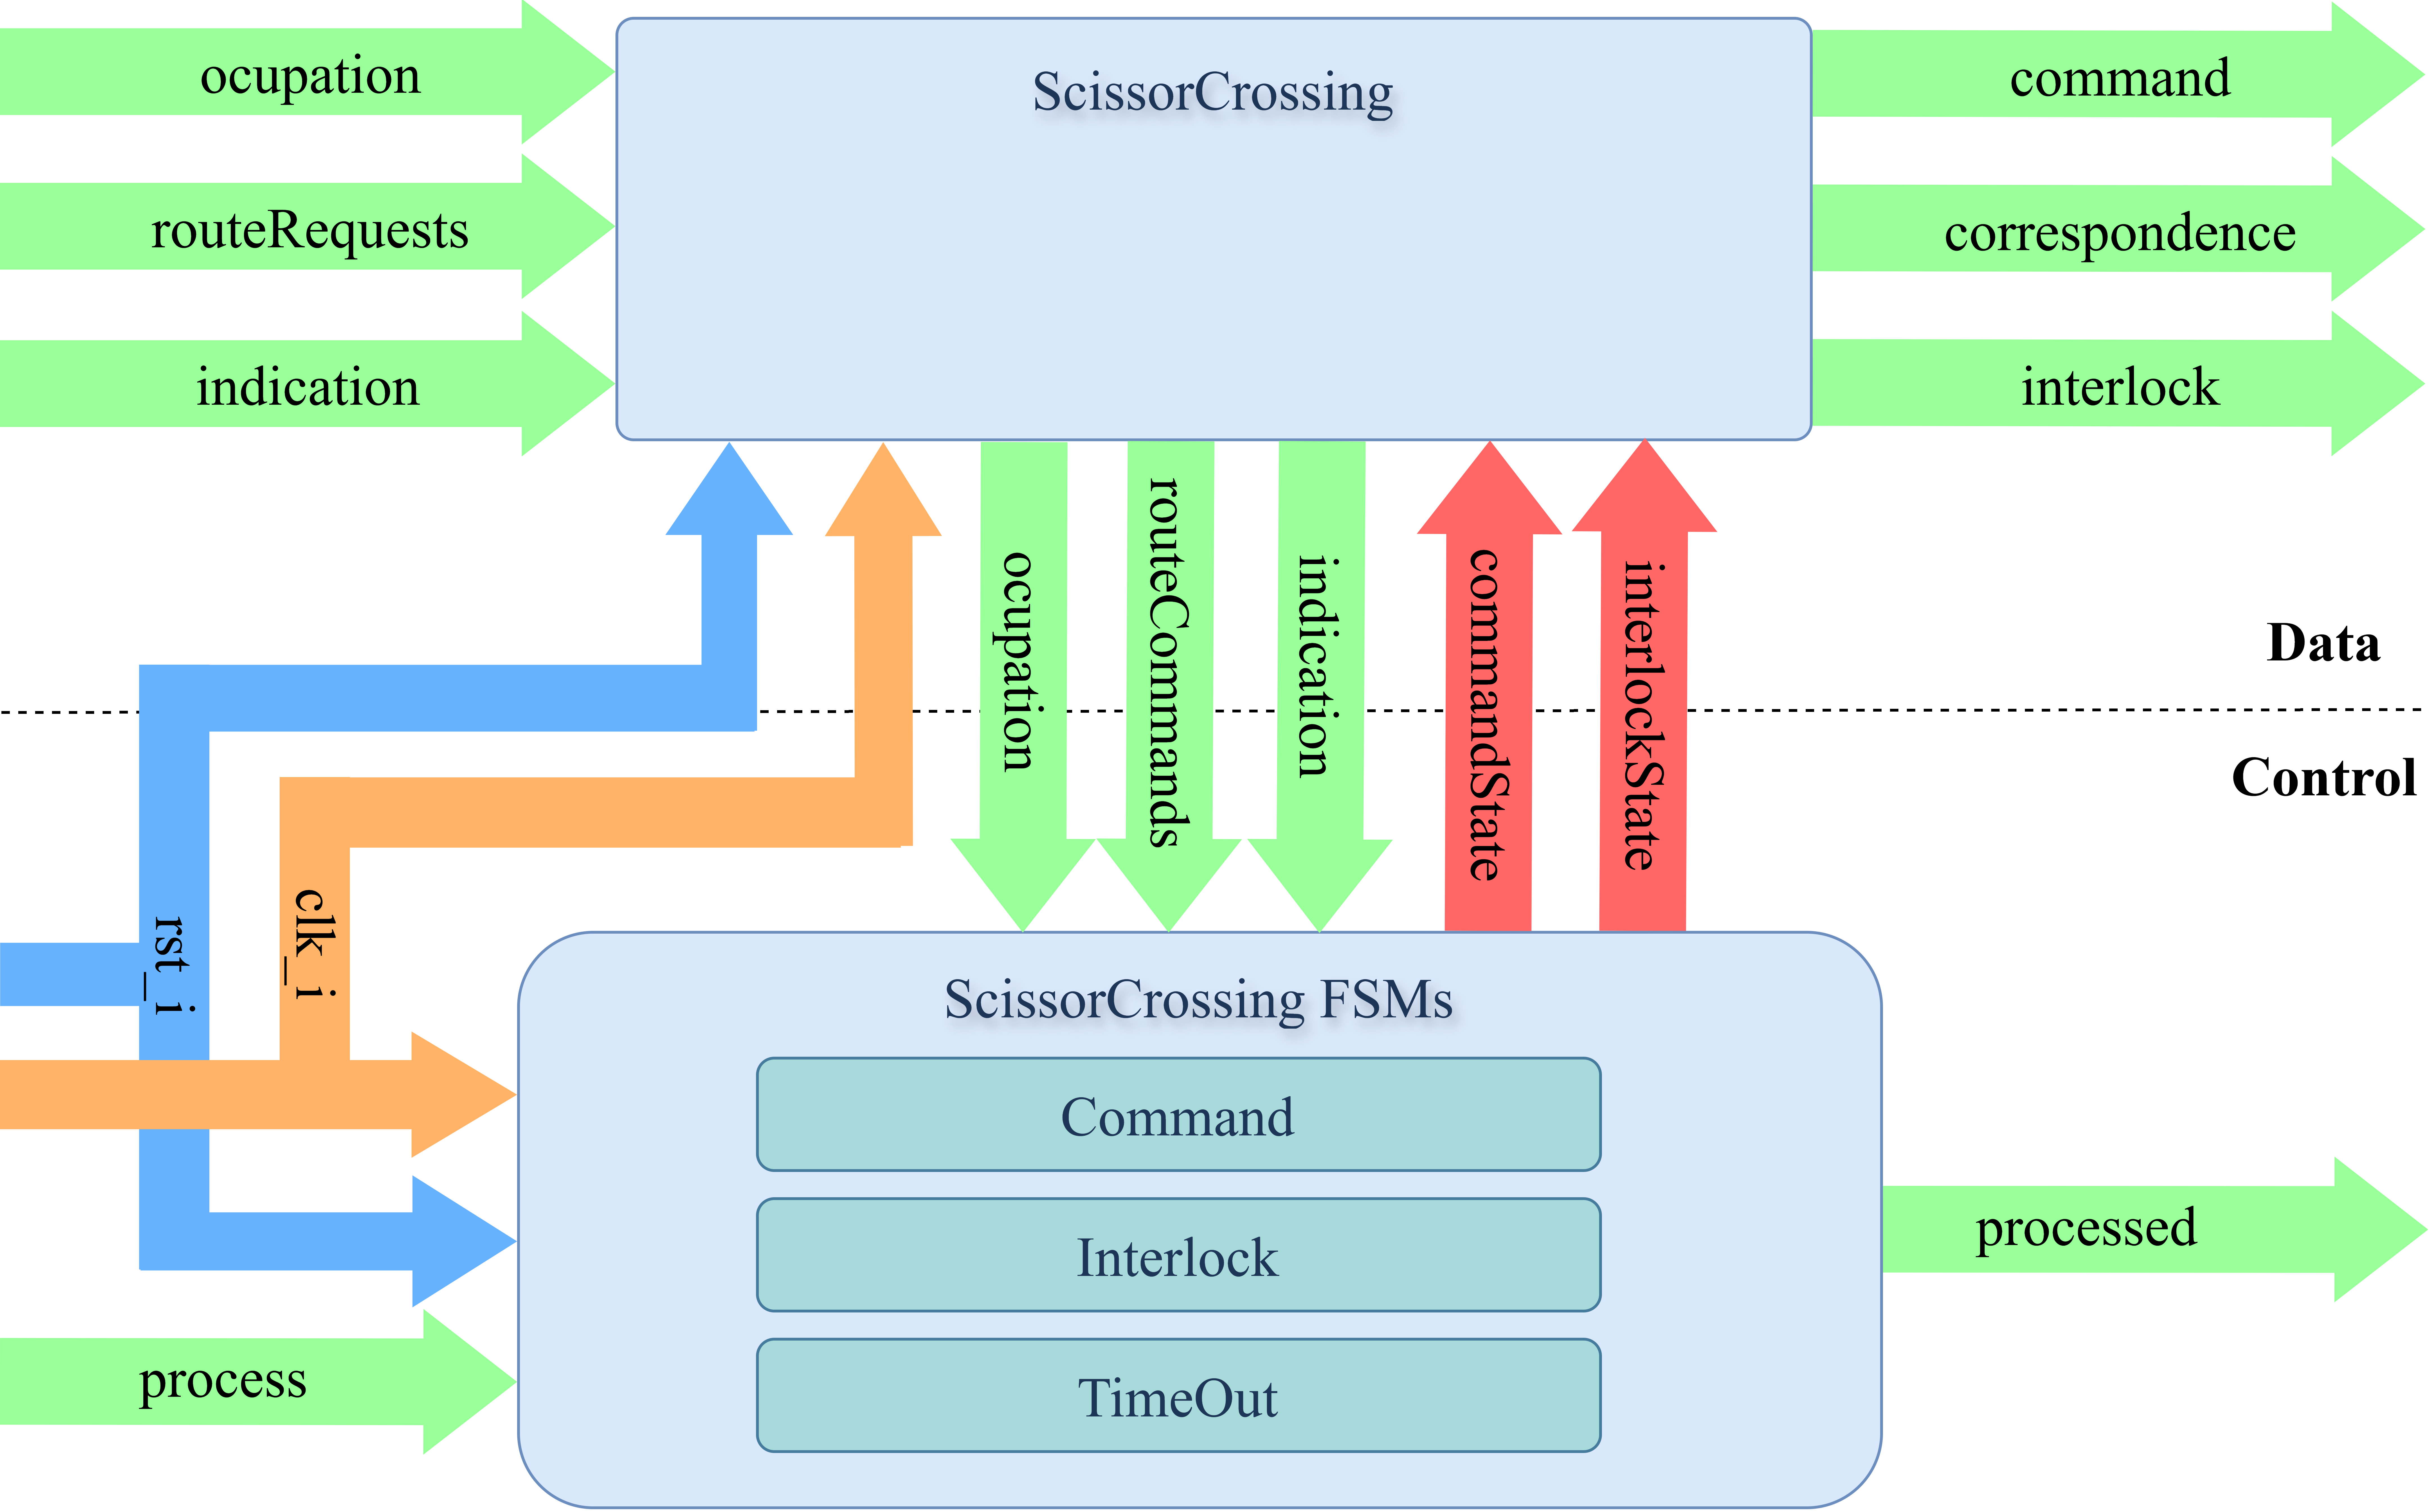
\includegraphics[width=1\textwidth]{Figuras/SCR_module}
	\centering\caption{FSMD del módulo genérico de \textit{ScissorCrossings}.}
	\label{fig:SCR_module}
\end{figure}

\lipsum[1]

\begin{figure}[H]
	\centering
	\includegraphics[width=1\textwidth]{Figuras/SSW_Petri}
	\centering\caption{Red de Petri del modelo dinámico de \textit{ScissorCrossings}.}
	\label{fig:SCR_Petri}
\end{figure}

\lipsum[1]
